% Created by tikzDevice version 0.12 on 2019-05-07 11:34:57
% !TEX encoding = UTF-8 Unicode
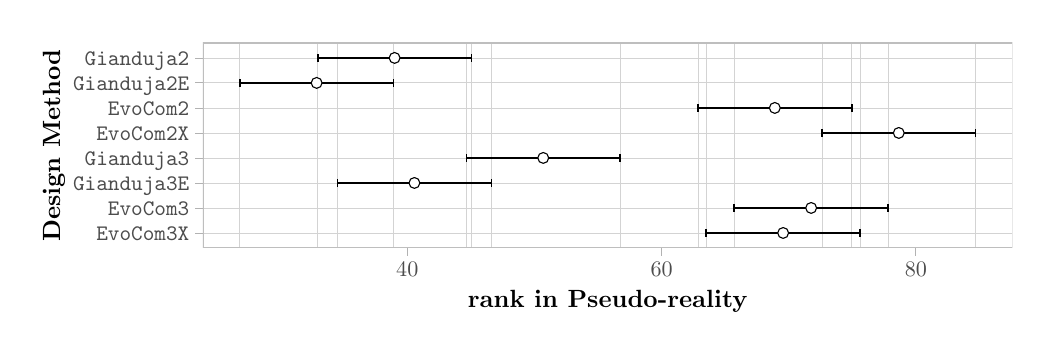
\begin{tikzpicture}[x=1pt,y=1pt]
\definecolor{fillColor}{RGB}{255,255,255}
\path[use as bounding box,fill=fillColor,fill opacity=0.00] (0,0) rectangle (361.35,108.41);
\begin{scope}
\path[clip] (  0.00,  0.00) rectangle (361.35,108.40);
\definecolor{drawColor}{RGB}{255,255,255}
\definecolor{fillColor}{RGB}{255,255,255}

\path[draw=drawColor,line width= 0.6pt,line join=round,line cap=round,fill=fillColor] (  0.00,  0.00) rectangle (361.35,108.40);
\end{scope}
\begin{scope}
\path[clip] ( 63.34, 28.81) rectangle (355.85,102.90);
\definecolor{fillColor}{RGB}{255,255,255}

\path[fill=fillColor] ( 63.34, 28.81) rectangle (355.85,102.90);
\definecolor{drawColor}{RGB}{211,211,211}

\path[draw=drawColor,line width= 0.3pt,line join=round] ( 63.34, 79.41) --
	(355.85, 79.41);

\path[draw=drawColor,line width= 0.3pt,line join=round] ( 63.34, 43.27) --
	(355.85, 43.27);

\path[draw=drawColor,line width= 0.3pt,line join=round] ( 63.34, 97.48) --
	(355.85, 97.48);

\path[draw=drawColor,line width= 0.3pt,line join=round] ( 63.34, 88.45) --
	(355.85, 88.45);

\path[draw=drawColor,line width= 0.3pt,line join=round] ( 63.34, 61.34) --
	(355.85, 61.34);

\path[draw=drawColor,line width= 0.3pt,line join=round] ( 63.34, 52.30) --
	(355.85, 52.30);

\path[draw=drawColor,line width= 0.3pt,line join=round] ( 63.34, 34.23) --
	(355.85, 34.23);

\path[draw=drawColor,line width= 0.3pt,line join=round] ( 63.34, 70.37) --
	(355.85, 70.37);

\path[draw=drawColor,line width= 0.2pt,line join=round] (297.76, 28.81) -- (297.76,102.90);

\path[draw=drawColor,line width= 0.2pt,line join=round] (342.55, 28.81) -- (342.55,102.90);

\path[draw=drawColor,line width= 0.2pt,line join=round] (310.89, 28.81) -- (310.89,102.90);

\path[draw=drawColor,line width= 0.2pt,line join=round] (300.77, 28.81) -- (300.77,102.90);

\path[draw=drawColor,line width= 0.2pt,line join=round] (132.20, 28.81) -- (132.20,102.90);

\path[draw=drawColor,line width= 0.2pt,line join=round] (160.37, 28.81) -- (160.37,102.90);

\path[draw=drawColor,line width= 0.2pt,line join=round] (167.54, 28.81) -- (167.54,102.90);

\path[draw=drawColor,line width= 0.2pt,line join=round] (214.08, 28.81) -- (214.08,102.90);

\path[draw=drawColor,line width= 0.2pt,line join=round] (242.20, 28.81) -- (242.20,102.90);

\path[draw=drawColor,line width= 0.2pt,line join=round] (286.99, 28.81) -- (286.99,102.90);

\path[draw=drawColor,line width= 0.2pt,line join=round] (255.32, 28.81) -- (255.32,102.90);

\path[draw=drawColor,line width= 0.2pt,line join=round] (245.21, 28.81) -- (245.21,102.90);

\path[draw=drawColor,line width= 0.2pt,line join=round] ( 76.64, 28.81) -- ( 76.64,102.90);

\path[draw=drawColor,line width= 0.2pt,line join=round] (104.81, 28.81) -- (104.81,102.90);

\path[draw=drawColor,line width= 0.2pt,line join=round] (111.97, 28.81) -- (111.97,102.90);

\path[draw=drawColor,line width= 0.2pt,line join=round] (158.52, 28.81) -- (158.52,102.90);
\definecolor{drawColor}{RGB}{0,0,0}

\path[draw=drawColor,line width= 0.6pt,line join=round] (297.76, 78.06) --
	(297.76, 80.77);

\path[draw=drawColor,line width= 0.6pt,line join=round] (297.76, 79.41) --
	(242.20, 79.41);

\path[draw=drawColor,line width= 0.6pt,line join=round] (242.20, 78.06) --
	(242.20, 80.77);

\path[draw=drawColor,line width= 0.6pt,line join=round] (342.55, 69.02) --
	(342.55, 71.73);

\path[draw=drawColor,line width= 0.6pt,line join=round] (342.55, 70.37) --
	(286.99, 70.37);

\path[draw=drawColor,line width= 0.6pt,line join=round] (286.99, 69.02) --
	(286.99, 71.73);

\path[draw=drawColor,line width= 0.6pt,line join=round] (310.89, 41.91) --
	(310.89, 44.62);

\path[draw=drawColor,line width= 0.6pt,line join=round] (310.89, 43.27) --
	(255.32, 43.27);

\path[draw=drawColor,line width= 0.6pt,line join=round] (255.32, 41.91) --
	(255.32, 44.62);

\path[draw=drawColor,line width= 0.6pt,line join=round] (300.77, 32.87) --
	(300.77, 35.59);

\path[draw=drawColor,line width= 0.6pt,line join=round] (300.77, 34.23) --
	(245.21, 34.23);

\path[draw=drawColor,line width= 0.6pt,line join=round] (245.21, 32.87) --
	(245.21, 35.59);

\path[draw=drawColor,line width= 0.6pt,line join=round] (132.20, 87.09) --
	(132.20, 89.80);

\path[draw=drawColor,line width= 0.6pt,line join=round] (132.20, 88.45) --
	( 76.64, 88.45);

\path[draw=drawColor,line width= 0.6pt,line join=round] ( 76.64, 87.09) --
	( 76.64, 89.80);

\path[draw=drawColor,line width= 0.6pt,line join=round] (160.37, 96.13) --
	(160.37, 98.84);

\path[draw=drawColor,line width= 0.6pt,line join=round] (160.37, 97.48) --
	(104.81, 97.48);

\path[draw=drawColor,line width= 0.6pt,line join=round] (104.81, 96.13) --
	(104.81, 98.84);

\path[draw=drawColor,line width= 0.6pt,line join=round] (167.54, 50.95) --
	(167.54, 53.66);

\path[draw=drawColor,line width= 0.6pt,line join=round] (167.54, 52.30) --
	(111.97, 52.30);

\path[draw=drawColor,line width= 0.6pt,line join=round] (111.97, 50.95) --
	(111.97, 53.66);

\path[draw=drawColor,line width= 0.6pt,line join=round] (214.08, 59.98) --
	(214.08, 62.69);

\path[draw=drawColor,line width= 0.6pt,line join=round] (214.08, 61.34) --
	(158.52, 61.34);

\path[draw=drawColor,line width= 0.6pt,line join=round] (158.52, 59.98) --
	(158.52, 62.69);

\path[draw=drawColor,line width= 0.4pt,line join=round,line cap=round,fill=fillColor] (269.98, 79.41) circle (  1.96);

\path[draw=drawColor,line width= 0.4pt,line join=round,line cap=round,fill=fillColor] (314.77, 70.37) circle (  1.96);

\path[draw=drawColor,line width= 0.4pt,line join=round,line cap=round,fill=fillColor] (283.11, 43.27) circle (  1.96);

\path[draw=drawColor,line width= 0.4pt,line join=round,line cap=round,fill=fillColor] (272.99, 34.23) circle (  1.96);

\path[draw=drawColor,line width= 0.4pt,line join=round,line cap=round,fill=fillColor] (104.42, 88.45) circle (  1.96);

\path[draw=drawColor,line width= 0.4pt,line join=round,line cap=round,fill=fillColor] (132.59, 97.48) circle (  1.96);

\path[draw=drawColor,line width= 0.4pt,line join=round,line cap=round,fill=fillColor] (139.75, 52.30) circle (  1.96);

\path[draw=drawColor,line width= 0.4pt,line join=round,line cap=round,fill=fillColor] (186.30, 61.34) circle (  1.96);
\definecolor{drawColor}{RGB}{190,190,190}

\path[draw=drawColor,line width= 0.6pt,line join=round,line cap=round] ( 63.34, 28.81) rectangle (355.85,102.90);
\end{scope}
\begin{scope}
\path[clip] (  0.00,  0.00) rectangle (361.35,108.41);
\definecolor{drawColor}{gray}{0.30}

\node[text=drawColor,anchor=base east,inner sep=0pt, outer sep=0pt, scale=  0.80] at ( 58.39, 76.66) {\texttt{EvoCom2}};

\node[text=drawColor,anchor=base east,inner sep=0pt, outer sep=0pt, scale=  0.80] at ( 58.39, 40.51) {\texttt{EvoCom3}};

\node[text=drawColor,anchor=base east,inner sep=0pt, outer sep=0pt, scale=  0.80] at ( 58.39, 94.73) {\texttt{Gianduja2}};

\node[text=drawColor,anchor=base east,inner sep=0pt, outer sep=0pt, scale=  0.80] at ( 58.39, 85.69) {\texttt{Gianduja2E}};

\node[text=drawColor,anchor=base east,inner sep=0pt, outer sep=0pt, scale=  0.80] at ( 58.39, 58.58) {\texttt{Gianduja3}};

\node[text=drawColor,anchor=base east,inner sep=0pt, outer sep=0pt, scale=  0.80] at ( 58.39, 49.55) {\texttt{Gianduja3E}};

\node[text=drawColor,anchor=base east,inner sep=0pt, outer sep=0pt, scale=  0.80] at ( 58.39, 31.48) {\texttt{EvoCom3X}};

\node[text=drawColor,anchor=base east,inner sep=0pt, outer sep=0pt, scale=  0.80] at ( 58.39, 67.62) {\texttt{EvoCom2X}};
\end{scope}
\begin{scope}
\path[clip] (  0.00,  0.00) rectangle (361.35,108.41);
\definecolor{drawColor}{gray}{0.70}

\path[draw=drawColor,line width= 0.3pt,line join=round] ( 60.59, 79.41) --
	( 63.34, 79.41);

\path[draw=drawColor,line width= 0.3pt,line join=round] ( 60.59, 43.27) --
	( 63.34, 43.27);

\path[draw=drawColor,line width= 0.3pt,line join=round] ( 60.59, 97.48) --
	( 63.34, 97.48);

\path[draw=drawColor,line width= 0.3pt,line join=round] ( 60.59, 88.45) --
	( 63.34, 88.45);

\path[draw=drawColor,line width= 0.3pt,line join=round] ( 60.59, 61.34) --
	( 63.34, 61.34);

\path[draw=drawColor,line width= 0.3pt,line join=round] ( 60.59, 52.30) --
	( 63.34, 52.30);

\path[draw=drawColor,line width= 0.3pt,line join=round] ( 60.59, 34.23) --
	( 63.34, 34.23);

\path[draw=drawColor,line width= 0.3pt,line join=round] ( 60.59, 70.37) --
	( 63.34, 70.37);
\end{scope}
\begin{scope}
\path[clip] (  0.00,  0.00) rectangle (361.35,108.41);
\definecolor{drawColor}{gray}{0.70}

\path[draw=drawColor,line width= 0.3pt,line join=round] (137.18, 26.06) --
	(137.18, 28.81);

\path[draw=drawColor,line width= 0.3pt,line join=round] (229.07, 26.06) --
	(229.07, 28.81);

\path[draw=drawColor,line width= 0.3pt,line join=round] (320.95, 26.06) --
	(320.95, 28.81);
\end{scope}
\begin{scope}
\path[clip] (  0.00,  0.00) rectangle (361.35,108.41);
\definecolor{drawColor}{gray}{0.30}

\node[text=drawColor,anchor=base,inner sep=0pt, outer sep=0pt, scale=  0.80] at (137.18, 18.35) {40};

\node[text=drawColor,anchor=base,inner sep=0pt, outer sep=0pt, scale=  0.80] at (229.07, 18.35) {60};

\node[text=drawColor,anchor=base,inner sep=0pt, outer sep=0pt, scale=  0.80] at (320.95, 18.35) {80};
\end{scope}
\begin{scope}
\path[clip] (  0.00,  0.00) rectangle (361.35,108.41);
\definecolor{drawColor}{RGB}{0,0,0}

\node[text=drawColor,anchor=base,inner sep=0pt, outer sep=0pt, scale=  0.90] at (209.60,  7.44) {\bfseries rank in Pseudo-reality};
\end{scope}
\begin{scope}
\path[clip] (  0.00,  0.00) rectangle (361.35,108.41);
\definecolor{drawColor}{RGB}{0,0,0}

\node[text=drawColor,rotate= 90.00,anchor=base,inner sep=0pt, outer sep=0pt, scale=  0.90] at ( 11.71, 65.86) {\bfseries Design Method};
\end{scope}
\end{tikzpicture}
